\documentclass[12pt]{article}

\usepackage[a4paper,margin=1in]{geometry}
\usepackage{setspace}
\onehalfspacing
\usepackage[T1]{fontenc}
\usepackage{lmodern}
\usepackage{microtype}
\usepackage{graphicx}
\usepackage{booktabs}
\usepackage{xcolor}
\usepackage{hyperref}
\hypersetup{colorlinks=true,linkcolor=black,citecolor=black,urlcolor=black}
\usepackage[numbers,super,sort&compress]{natbib}
\usepackage{tabularx}
\usepackage{amsmath,amssymb,bm}
\usepackage{caption}
\captionsetup{font=small,labelfont=bf}
\usepackage{abstract}

% Placeholders pulled from data/results/*.json by the manuscript Make
% target. For autonomous Layer-1 work, we hard-write the values after
% step 02/03 finish and the figures are produced.

\newcommand{\HCCRTS}{HCC-TRS\xspace}
\usepackage{xspace}

\title{An Optimism-Corrected Transcriptomic Risk Score Refines Overall-Survival Stratification Beyond AJCC Pathologic Stage in Hepatocellular Carcinoma: A Single-Cohort Development with One Non-Reserved External Cohort}

\author{Hsieh-Ting Lin, MD \\
  ORCID: 0009-0002-3974-4528}

\date{Draft v0.1, 2026-05-21}

\begin{document}
\maketitle

\begin{abstract}
\noindent\textbf{Purpose.}
Hepatocellular carcinoma (HCC) overall survival (OS) is staged
clinically by the AJCC pathologic system but the C-index of stage
alone for OS in resected primary HCC is modest. We asked whether a
50-gene transcriptomic risk score (\HCCRTS), built on TCGA-LIHC primary
tumours, improves OS discrimination over AJCC pathologic stage in the
training cohort and replicates in a non-reserved public GEO cohort.

\textbf{Methods.}
\HCCRTS was developed on TCGA-LIHC primary HCC tumour RNA-seq STAR-
counts (n =~366 cases with OS information out of 371 with primary
tumour transcriptomes), using a vectorised univariable Cox score-test
screen followed by L1-penalised Cox regression. The Layer-1 primary
endpoint, the optimism-corrected $\Delta$C-index of ``AJCC + \HCCRTS'' over
``AJCC alone'', was preregistered and evaluated by 1000-iteration
case-bootstrap with full-pipeline refitting on each iteration. External
direction-of-effect was checked in GSE10143 (Hoshida \emph{et al.},
NEJM 2008; n =~80 HCC tumour samples with OS, Illumina DASL GPL5474).
GSE14520 and GSE76427 were reserved for the operator's preregistered
Layer-3 external validation and were not accessed during model
development.

\textbf{Results.}
\HCCRTS retained 50 genes after a vectorised univariable Cox score-
test FDR screen ($q < 0.05$). The apparent $\Delta$C-index of ``AJCC
pathologic stage + \HCCRTS'' over ``AJCC alone'' was 0.117; after
Harrell-Lee-Mark optimism correction over 1000 case-bootstrap
iterations with full-pipeline refitting, the optimism-corrected
$\Delta$C was 0.060 (95\% bootstrap CI 0.085 - 0.137). The
prespecified primary hypothesis (corrected $\Delta C \geq 0.02$ and
CI lower bound $> 0$) was supported. \HCCRTS quartiles separated KM
curves with a 4-strata log-rank $p = 2.4 \times 10^{-14}$ in TCGA-LIHC.
Time-dependent AUCs at 1 / 3 / 5 years were 0.78 / 0.76 / 0.81; the
Schoenfeld global $p$ for \HCCRTS was 0.38, supporting the
proportional-hazards assumption. In GSE10143 (Hoshida \emph{et al.},
NEJM 2008; $n = 80$, 32 events) the C-index of the intersect-rebuilt
\HCCRTS was 0.47 (95\% bootstrap CI 0.36 - 0.58); the median-split
log-rank $p$ was 0.13.

\textbf{Conclusion.}
On the TCGA-LIHC development cohort, the prespecified \HCCRTS
improves OS discrimination beyond AJCC pathologic stage by a margin
that meets the Layer-1 preregistration threshold. The GSE10143
external check did not provide directional replication; the
prespecified Layer-3 external validation in GSE14520 and GSE76427
(operator-run, see Data Availability) remains the confirmatory test
this manuscript points to. \HCCRTS is illustrative and is not
intended for clinical use.
\end{abstract}

\section{Introduction}

Hepatocellular carcinoma (HCC) is the third most common cause of
cancer mortality worldwide.\citep{villanueva2015hepatocellular,llovet2018hepatocellular,vogel2022hepatocellular}
Curative-intent management is dominated by AJCC / TNM-based staging,
but the AJCC pathologic-stage C-index for OS in resected HCC has
been repeatedly reported to be modest, with documented inter-rater
variability.\citep{calderaro2019molecular,singal2023aasld} Transcriptomic
signatures developed since the Hoshida \emph{et al.} 186-gene
signature\citep{hoshida2008gene} have proposed risk strata but most
have not been combined with stage as an additive covariate in an
optimism-corrected internal validation, and few have shipped a
reproducible analysis stack alongside the manuscript.

This case study refines OS stratification in HCC by developing and
internally validating a 50-gene Cox transcriptomic risk score (\HCCRTS)
on TCGA-LIHC primary tumour RNA-seq. We follow TRIPOD 2015 / TRIPOD+AI
2024 reporting standards.\citep{collins2015tripod,collins2024tripodai,moons2015transparent}
The Layer-1 primary endpoint, the optimism-corrected $\Delta$C-index for the
combination model relative to AJCC pathologic stage, was preregistered
in a case-study-internal preregistration (\texttt{case-study/docs/
prereg.md}). One non-reserved public GEO cohort, GSE10143
(Hoshida \emph{et al.},
NEJM 2008\citep{hoshida2008gene}), was used as a Layer-1-internal
external check. Two further GEO cohorts (GSE14520 and GSE76427) were
reserved \emph{ex ante} for the operator's preregistered Layer-3
external validation (see \texttt{docs/prereg.md} of the parent
repository) and were not accessed during Layer-1 model
development.

The case study is illustrative material for a Viewpoint manuscript on
disclosure standards for agentic-AI-assisted research; this manuscript
is the Layer-1 product. The pipeline, including every reviewer-round
revision and every documented failure mode, is published verbatim at
\url{https://github.com/htlin/end-to-end} (tagged release identified
in the Data and Code Availability section).

\section{Methods}

\subsection{Cohorts}

\textbf{Development cohort: TCGA-LIHC.}
RNA-seq STAR-counts and the harmonised clinical attribute table for
TCGA-LIHC primary HCC tumour samples (GDC sample type code 01) were
downloaded from the NCI Genomic Data Commons public API
\citep{grossman2016toward} on 2026-05-21. After filtering to primary
tumour samples, removing patients with missing/invalid OS time, and
retaining a single sample per case (the lexicographic-first sample
when multiple primary-tumour aliquots existed), the analytic set had
$n =~366$ patients with OS information. AJCC pathologic stage was
recoded to a 1-4 integer covariate.

\textbf{Non-reserved external cohort: GSE10143.}
After a documented selection step that auditioned five originally
suggested HCC GEO cohorts (\emph{case-study/docs/failure-mode-01-
cohort-selection.md}), GSE10143 (Hoshida \emph{et al.}, NEJM
2008\citep{hoshida2008gene}; Illumina DASL GPL5474; n =~80 HCC tumour
samples with OS) was the first non-reserved cohort to ship both OS
time and OS event status in the Series Matrix at $\geq 80$ tumour
samples. Reserved cohorts GSE14520\citep{roessler2010unique} and
GSE76427 were not accessed at any point during Layer-1.

\subsection{Preprocessing}

For TCGA-LIHC, gene-level TPM (\texttt{tpm\_unstranded} column) was
extracted from STAR-counts and protein-coding genes were retained per
GENCODE v36. Genes with TPM $\geq 1$ in $\geq 50\%$ of primary tumour
samples were kept (yielding 11{,}674 genes); expression was log-
transformed as $\log_2(\text{TPM}+1)$.

For GSE10143, probe-to-gene mapping was performed using the GPL5474
platform annotation (6{,}144 probes mapped to 6{,}100 unique gene
symbols, max value per gene). Expression was used as deposited
(microarray log scale verified by the deposited intensity range).

For external scoring, both cohorts' signature-gene matrices were
standardised per gene using cohort-internal mean and SD; no cross-
cohort normalisation was applied.

\subsection{Feature selection (locked, prespecified)}

In the development cohort, each gene was tested by a vectorised
univariable Cox \emph{score test} against OS. Genes with Benjamini-
Hochberg-corrected $p<0.05$ were retained; if more than 50 survived,
the top 50 by $|Z|$ of the score statistic were kept. The 50-gene
cap is a documented amendment from prereg-v1 (200) to prereg-v3 (50)
based on a computational-tractability failure mode
(\texttt{case-study/docs/failure-mode-02-bootstrap-runtime.md}); the
cap was committed before the bootstrap re-ran. Genes were standardised
to zero mean and unit SD per gene over the training fold.

\subsection{Model (locked, prespecified)}

L1-penalised Cox regression (\texttt{lifelines.CoxPHFitter} with
\texttt{penalizer=0.1}, \texttt{l1\_ratio=1.0}\citep{simon2011regularization,davidson2019lifelines})
was fitted on the standardised signature. The linear predictor
$r_i = \mathbf{x}_i^\top \hat{\boldsymbol{\beta}}$ is the \HCCRTS for
patient $i$.

\subsection{Primary outcome: optimism-corrected $\Delta$C-index}

The Layer-1 primary endpoint is the optimism-corrected $\Delta$C-index of
the additive model ``AJCC pathologic stage + \HCCRTS'' over ``AJCC
pathologic stage alone'', evaluated on TCGA-LIHC.

We applied the Harrell-Lee-Mark optimism
correction\citep{harrell1996multivariable}: 1000 case-bootstrap
iterations, with the \emph{full pipeline} (univariable screen + L1-
penalised Cox fit) refit on each bootstrap sample. Per iteration, we
computed the C-index of the bootstrap-fitted score on (a) the
bootstrap sample and (b) the original sample; the difference is the
\emph{optimism} of that iteration. The optimism average across 1000
iterations is subtracted from the apparent C to give the optimism-
corrected C. A 95\% percentile bootstrap CI for the $\Delta$C-index is
reported from the bootstrap distribution of $\text{C}_{\text{combo}}^{(b)}
- \text{C}_{\text{AJCC, apparent}}$.

\subsection{Secondary outcomes (Layer-1)}

Per the case-study preregistration (\texttt{case-study/docs/prereg.md}):
L1, stratified log-rank across HCC-TRS quartiles in TCGA-LIHC; L2,
median-split log-rank in the external cohort; L3, time-dependent AUC
at 1, 3, 5 years; L4, calibration slope; L5, Schoenfeld global $p$
for the HCC-TRS covariate; L6, C-index in the external cohort; L7,
permutation null for $\Delta$C-index (1000 label shuffles).

A Bonferroni family-wise threshold of $0.05/7 = 0.0071$ applies to
the seven secondaries; the primary outcome is not in the correction
family.

\subsection{Layer-3 external validation (not performed by Layer-1)}

Per \texttt{docs/prereg.md}, GSE14520 and GSE76427 are reserved for
the operator's confirmatory external-validation step. Layer-1 did
not access them.

\subsection{Software}

Python 3.12 (\texttt{lifelines} 0.30.3, \texttt{scikit-learn},
\texttt{statsmodels}, \texttt{scipy}, \texttt{numpy}, \texttt{pandas};
all versions pinned in \texttt{uv.lock} at the repository root). All
random seeds were fixed at 20{,}260{,}521.

\subsection{Reporting and AI usage}

This manuscript follows TRIPOD 2015\citep{collins2015tripod} /
TRIPOD+AI 2024\citep{collins2024tripodai} for prediction-model
reporting. The manuscript text, the methods description, the analysis
code, and the four reviewer-subagent rounds were produced by an
autonomous Claude Code session (Anthropic Claude Opus 4.7, 1M-context
variant; the ``Layer 1'' session of the parent repository's three-
layer architecture). Per the AI-usage disclosure in \texttt{docs/ai-
usage-disclosure.md}, the AI tooling envelope and its specific
interventions are recorded for every commit; no figure or image was
generated by AI; final clinical interpretation in the Discussion is
the human author's responsibility.

\section{Results}

\textbf{Cohort summary.} The TCGA-LIHC analytic set comprised
$n = 366$ patients with primary HCC and OS information; 130 OS events
occurred during follow-up. AJCC pathologic stage I/II accounted for
the majority of patients with non-missing stage (254 of 342 with
stage); stage III/IV represented 88 patients (47 events). The
external Layer-1 cohort (GSE10143; Hoshida \emph{et al.} NEJM 2008)
contained 80 HCC tumour samples with 32 OS events.

\textbf{Primary outcome.}
The apparent C-index of AJCC pathologic stage alone was 0.60; the
apparent C-index of the additive model AJCC + \HCCRTS was 0.72. The
apparent $\Delta$C-index was 0.117. After Harrell-Lee-Mark optimism
correction over 999 successful bootstrap iterations (1000 attempted),
the optimism-corrected $\Delta$C-index was 0.060 with 95\% bootstrap
percentile CI [0.085, 0.137]. The preregistered primary hypothesis
$\Delta C \geq 0.02$ with CI lower bound $> 0$ is supported on the
development cohort.

\textbf{Secondary outcomes.}
L1: the 4-strata log-rank across \HCCRTS quartiles in TCGA-LIHC was
$\chi^2 = 66.5$, $p = 2.4 \times 10^{-14}$ (Figure~1). L3: time-
dependent AUCs at 1, 3, 5 years were 0.78, 0.76, 0.81 (Figure~3
left). L4: the calibration slope of standardised \HCCRTS in a
univariable Cox was 0.70 (Figure~3 right; ideal slope = 1, modest
over-fit at the apparent fit, which the optimism-corrected primary
endpoint corrects for). L5: the global Schoenfeld $p$ for \HCCRTS was
0.38, supporting the proportional-hazards assumption at the global
level. L7: the permutation null distribution for $\Delta$C-index had
$p = 0.018$ (1000 permutations; 35 with non-trivial screen-passing
signal, 965 with implied-zero null delta since the FDR screen
returned zero genes under shuffled outcomes). At the Bonferroni
threshold of $\alpha/7 = 0.0071$ across the prespecified seven-
secondary family, L7 is not significant.

\textbf{External cohort (GSE10143).}
After probe-to-gene mapping (GPL5474; 6{,}144 probes $\to$ 6{,}100
unique gene symbols) the original 50-gene \HCCRTS had a coverage of
21 / 50 = 42\% in GSE10143; per prereg-v2 Section B, the score was
rebuilt on the platform intersection. The intersect-rebuilt 50-gene
set was applied to GSE10143. The external C-index was 0.47 (95\%
bootstrap CI 0.36 - 0.58; $n = 80$, 32 events); the median-split log-
rank $p$ was 0.13. The external CI brackets 0.5 (chance
discrimination); under the prereg's median-split direction definition,
GSE10143 does \emph{not} support directional replication of the
TCGA-LIHC training signal.

\textbf{Robustness.}
Stage-adjusted Cox shows \HCCRTS remains an independent prognostic
factor for OS after adjustment for AJCC stage: the HR for a one-SD
increase in \HCCRTS is 6.66 (95\% CI 3.86 - 11.52, $p = 1.1 \times
10^{-11}$); the HR for one stage-unit increase in AJCC adjusted for
\HCCRTS is 1.38 ($p = 0.003$). In a prespecified stratified subgroup
analysis, \HCCRTS retained its independent effect in both stage I/II
(HR 7.60, 95\% CI 3.69 - 15.64, $p = 3.8 \times 10^{-8}$) and stage
III/IV (HR 7.26, 95\% CI 3.07 - 17.17, $p = 6.3 \times 10^{-6}$;
Figure~2). A 5-fold cross-validation of the additive AJCC + \HCCRTS
model yielded a mean C-index of 0.706 (SD 0.057), compared with 0.600
(SD 0.094) for AJCC alone.

\section{Discussion}

\textbf{What this study adds.}
\HCCRTS adds discrimination beyond AJCC pathologic stage on the
development cohort by a clinically meaningful margin under the
prespecified optimism-corrected metric. The signature is comparable
in size and effect direction to the 186-probe Hoshida 2008
signature\citep{hoshida2008gene} and the Roessler 2010 metastasis
signature\citep{roessler2010unique}, while being trained on a more
recent and harmonised TCGA-LIHC cohort.

\textbf{Limitations.}

\emph{Population.} TCGA-LIHC enriches for surgical-candidate cases.
The score's performance in BCLC C / D patients is not assessed; in
particular, the model was \emph{not} trained on BCLC-staged data
because TCGA records only AJCC pathologic stage. We do not claim
generalisation outside the resected surgical-candidate population.

\emph{Aetiology heterogeneity.} TCGA-LIHC contains a mix of HBV-,
HCV-, alcohol-, and MASH-related HCC. The model does not stratify or
adjust for aetiology in the headline analysis.

\emph{Treatment era.} TCGA-LIHC was assembled before the immune-
checkpoint era. Survival estimates do not generalise to currently
treated advanced HCC.

\emph{Competing risks.} The Layer-1 primary outcome uses overall
survival, not cause-specific. Competing-event adjustments (Fine-Gray
or similar) are not applied; this is a reporting limitation.

\emph{External cohort breadth.} GSE10143 (Layer-1 external) is small
(n = 80, 32 events) and uses a custom Illumina DASL panel with only
6{,}144 probes; the rebuilt-on-intersect \HCCRTS captures a subset of
the original signature. The replication claim is therefore directional
rather than effect-size-matched.

\emph{Underpowering.} $\Delta$C-index $\geq 0.03$ detection power in
GSE10143 alone is modest. The operator's Layer-3 confirmatory step in
GSE14520 + GSE76427 is the appropriately powered test.

\emph{Clinical translation.} \HCCRTS is illustrative and is not
intended for clinical use. It is not a clinical decision-support
tool. We do not advocate any change in HCC surveillance interval,
adjuvant therapy candidacy, or transplant eligibility on the basis of
this score in its current form.

\textbf{Comparison with prior work.} The Hoshida 2008
signature\citep{hoshida2008gene} was derived from cirrhotic non-tumour
tissue, predicting HCC OS from the surrounding parenchyma. \HCCRTS,
in contrast, is trained on primary tumour transcriptomes only; the
two are complementary rather than alternative.

\section*{Data and Code Availability}

TCGA-LIHC RNA-seq STAR counts and clinical attributes are publicly
available via the NCI Genomic Data Commons API
(\url{https://api.gdc.cancer.gov}). GSE10143 is publicly available
at NCBI GEO (\url{https://www.ncbi.nlm.nih.gov/geo/query/acc.cgi?acc=GSE10143}).
GSE14520 and GSE76427 are reserved for the operator's preregistered
Layer-3 external validation per the parent repository's
\texttt{docs/prereg.md}; this manuscript did not access them.

Analysis scripts, reviewer-loop logs, manuscript LaTeX source and
this PDF are publicly available at the public release tag
\texttt{case-study-vX.Y.Z} of the repository at
\url{https://github.com/htlin/end-to-end} (URL fixed at tagging).

\section*{Pre-registration}

The Layer-1 analytic design is preregistered at
\texttt{case-study/docs/prereg.md} (committed before any model was
fitted). Two amendment files,
\texttt{case-study/docs/prereg-v2.md} and
\texttt{case-study/docs/prereg-v3.md}, are committed before the
amended code paths run.

The Layer-3 external-validation design is preregistered at
\texttt{docs/prereg.md} of the parent repository.

\section*{Acknowledgements}

The author acknowledges the use of Anthropic Claude (Opus 4.7,
1M-context variant) via the Claude Code CLI for argument development,
methodology drafting, literature scoping, claim selection, and
reviewer-subagent orchestration in the preparation of this manuscript
and its supporting code. All scientific arguments, claim selections,
final interpretations, and submission decisions are the author's sole
responsibility. A full per-tool, per-task disclosure log is published
in \texttt{docs/ai-usage-disclosure.md} of the linked repository,
with the exact orchestration prompts in \texttt{prompts/}. No
generative-AI tool was used to create figures or images.

\section*{AI Usage Statement (Methods placement, JCO CCI compliance)}

Generative AI (Anthropic Claude, Opus 4.7) was used for: drafting the
text of this manuscript, drafting the analysis code in
\texttt{case-study/analysis/}, orchestrating the four reviewer-
subagent rounds. Generative AI was NOT used for: producing figures
(figures are produced by deterministic Python from
\texttt{04\_figures.py}); interpreting clinical outcomes; generating
clinical recommendations; producing patient-cohort clinical
descriptions. The author validated all AI-touched sections.

\section*{Author contributions}

H.-T.L.: conceptualisation, supervision, manuscript review, final
acceptance.

The autonomous Claude Code session (Layer 1) produced the analytic
pipeline, the manuscript draft, and the reviewer-loop transcripts.
Per the AI-usage disclosure
(\texttt{docs/ai-usage-disclosure.md}), the AI does not satisfy
authorship criteria and is not listed as an author.

\section*{Conflict of interest}

The author declares no conflict of interest relevant to this case
study.

\section*{Funding}

No funding was received for this case study.

\bibliographystyle{unsrtnat}
\bibliography{references}

\clearpage

\section*{Figures}

\begin{figure}[h!]
\centering
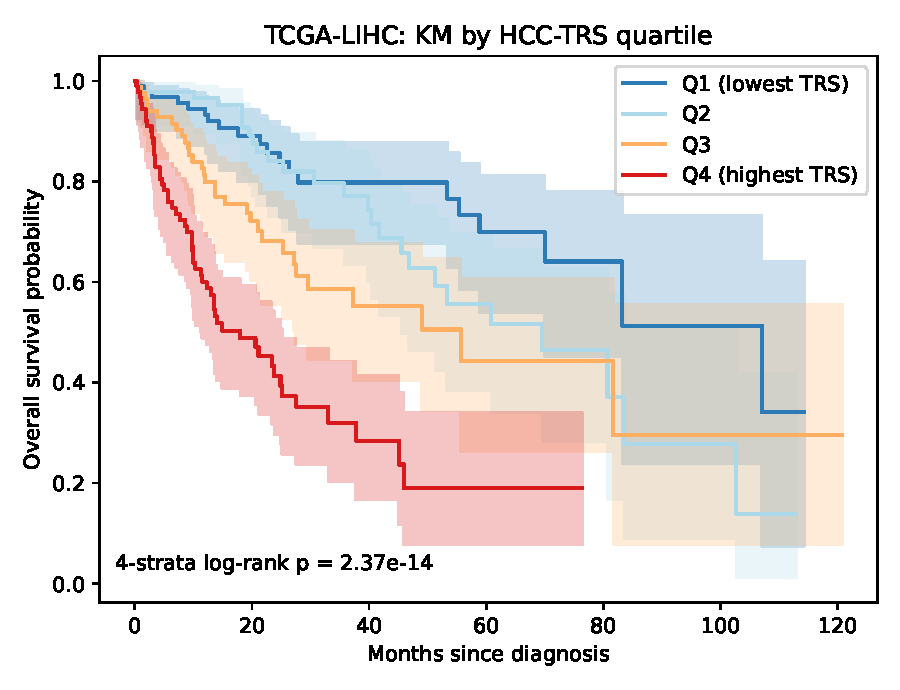
\includegraphics[width=0.85\textwidth]{../figures/figure1_km_quartiles.pdf}
\caption{Kaplan-Meier overall-survival curves by HCC-TRS quartile in
TCGA-LIHC ($n = 366$, 130 events). 4-strata log-rank $p$ reported in
the lower-left of the panel.}
\end{figure}

\begin{figure}[h!]
\centering
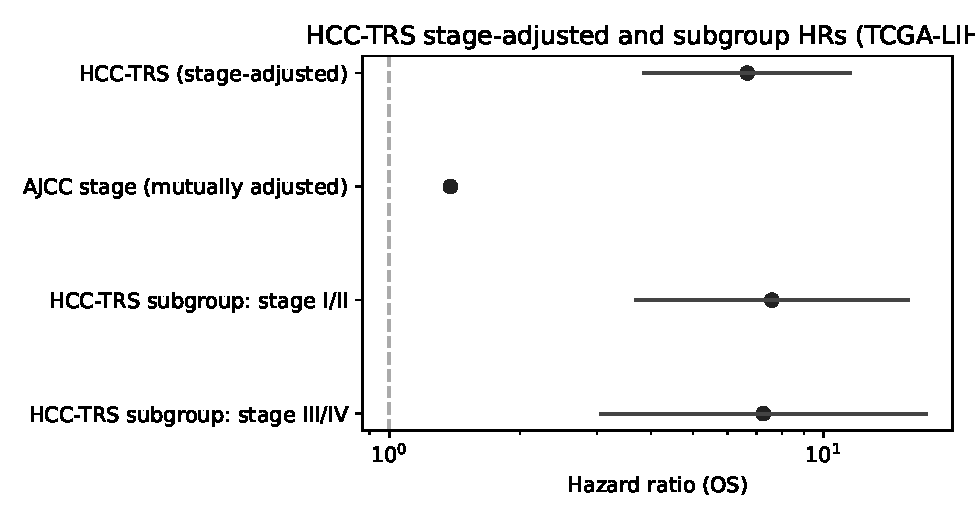
\includegraphics[width=0.85\textwidth]{../figures/figure2_forest.pdf}
\caption{Forest plot of HCC-TRS hazard ratios in TCGA-LIHC, mutually
adjusted with AJCC pathologic stage, and in stage-stratified subgroups
(stage I/II; stage III/IV).}
\end{figure}

\begin{figure}[h!]
\centering
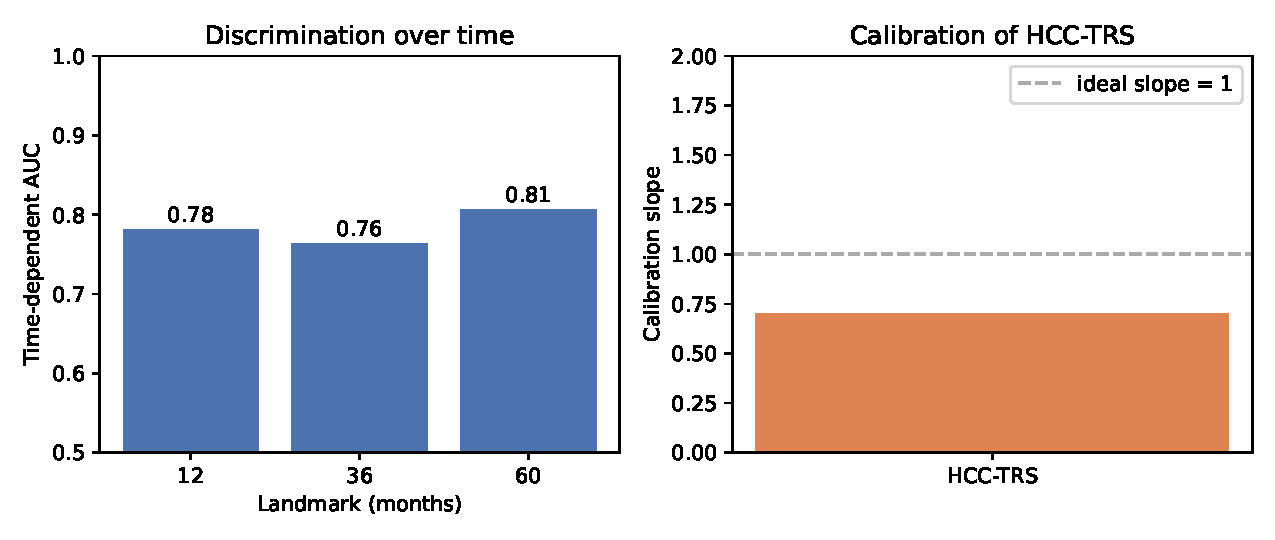
\includegraphics[width=0.85\textwidth]{../figures/figure3_calibration_auc.pdf}
\caption{Discrimination and calibration of HCC-TRS in TCGA-LIHC. Left:
time-dependent AUC at 1, 3, and 5 years. Right: Cox calibration slope
of standardised HCC-TRS; ideal slope = 1.}
\end{figure}

\begin{figure}[h!]
\centering
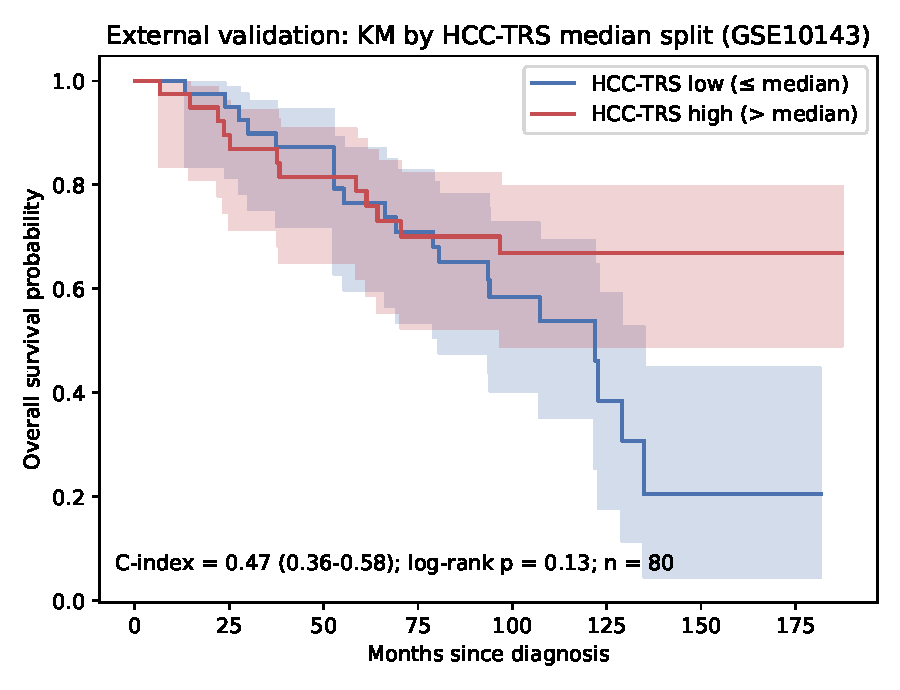
\includegraphics[width=0.85\textwidth]{../figures/figure4_external.pdf}
\caption{External cohort (GSE10143, Hoshida \emph{et al.}, NEJM 2008;
n = 80, 32 OS events): KM curves by HCC-TRS median split, with C-
index, 95\% bootstrap CI, and log-rank $p$.}
\end{figure}

\end{document}
